\chapter{Mendix}
%    Στο κεφάλαιο αυτό θα αναλυθεί το Mendix, μία από τις πιο διαδεδομένες πλατφόρμες ανάπτυξης λογισμικού που βασίζεται στην προσέγγιση low-code. Θα παρουσιαστούν οι βασικές λειτουργίες της πλατφόρμας, καθώς και οι δυνατότητες που προσφέρει στους χρήστες της.

    \section{Τι είναι το Mendix;}
        Το Mendix αποτελεί μία από τις πιο διαδεδομένες και καινοτόμες πλατφόρμες ανάπτυξης λογισμικού που βασίζεται στην προσέγγιση low-code. Ανήκει στις πλατφόρμες που επιτρέπουν την ταχύτερη και πιο αποδοτική ανάπτυξη εφαρμογών χωρίς να απαιτείται εκτενής γνώση προγραμματιστικών γλωσσών, γεγονός που καθιστά τη διαδικασία προσβάσιμη σε χρήστες με περιορισμένη ή καθόλου τεχνική κατάρτιση. Ιδρύθηκε το 2005 στο Ρότερνταμ της Ολλανδίας με στόχο να παρέχει στους επιχειρηματίες και τους οργανισμούς τη δυνατότητα να αναπτύσσουν, να προσαρμόζουν και να διαχειρίζονται εφαρμογές γρήγορα, με ελάχιστο κόστος και χωρίς την ανάγκη περίπλοκων κωδικοποιητικών διαδικασιών.

        Η καινοτομία του Mendix έγκειται στην εξαιρετική ευχρηστία του περιβάλλοντος ανάπτυξης, το οποίο ενσωματώνει εργαλεία drag-and-drop και visual modeling, επιτρέποντας στους χρήστες να δημιουργούν ολοκληρωμένες εφαρμογές χωρίς να χρειάζεται να κατανοούν σε βάθος τον προγραμματισμό. Αυτό το χαρακτηριστικό έχει συμβάλλει σημαντικά στην εξάπλωσή του, καθώς δίνει τη δυνατότητα σε επαγγελματίες από διάφορους τομείς, όπως μάρκετινγκ, οικονομικά και ανθρώπινο δυναμικό, να συμμετέχουν ενεργά στη διαδικασία ανάπτυξης εφαρμογών.

        Το 2018, το Mendix εξαγοράστηκε από την Siemens, τη μεγαλύτερη βιομηχανική κατασκευαστική εταιρεία στην Ευρώπη, γεγονός που επέφερε σημαντικές εξελίξεις στην πλατφόρμα. Η συγχώνευση αυτή επέτρεψε την ενσωμάτωση προηγμένων βιομηχανικών και IoT (Internet of Things) λύσεων, ενισχύοντας τη θέση του Mendix στην αγορά του λογισμικού επιχειρηματικής εφαρμογής. Μέσω αυτής της συνεργασίας, η Siemens κατάφερε να επωφεληθεί από τις δυνατότητες της low-code πλατφόρμας για να επιταχύνει τη δημιουργία βιομηχανικών εφαρμογών και να προωθήσει τον ψηφιακό μετασχηματισμό στον τομέα της βιομηχανίας.

        Η πλατφόρμα Mendix παρέχει ολοκληρωμένες δυνατότητες, όχι μόνο για την ανάπτυξη αλλά και για την ανάπτυξη cloud-based εφαρμογών, υποστηρίζοντας το DevOps μοντέλο για καλύτερη συνεργασία μεταξύ των ομάδων ανάπτυξης και παραγωγής. Η δυνατότητα ενσωμάτωσης με άλλες τεχνολογίες και συστήματα, καθώς και η ευκολία στην προσαρμογή της πλατφόρμας στις ανάγκες του εκάστοτε χρήστη, ενδυναμώνει τη δημοτικότητά της σε παγκόσμιο επίπεδο.

        Έτσι, το Mendix αποτελεί μία από τις πιο ισχυρές και ευέλικτες λύσεις στην αγορά του low-code προγραμματισμού, προσφέροντας αποτελεσματικότητα, ταχύτητα και καινοτομία στην ανάπτυξη λογισμικού, ενώ παράλληλα ενσωματώνει τις πιο σύγχρονες τεχνολογίες για να καλύψει τις ανάγκες επιχειρήσεων που επιθυμούν να παραμείνουν ανταγωνιστικές στην ψηφιακή εποχή.

        \cite{LowCodeMendix}


%        Το Mendix είναι από τις δημοφιλέστερες πλατφόρμες ανάπτυξης λογισμικού σε low-code. Η εταιρία ιδρύθηκε στο Ρότερνταμ της Ολλανδίας το 2005 με σκοπό τη δημιουργία μιας πλατφόρμας έτσι ώστε οι επιχειρήσεις να μπορούν να αναπτύσσουν εφαρμογές γρήγορα και αποδοτικά. Το 2018 εξαγοράστηκε από τη Siemens, τη μεγαλύτερη βιομηχανική κατασκευαστική εταιρία στην Ευρώπη, κάτι που επέτρεψε να γίνουν ενσωματώσεις και βελτιώσεις σε σύντομο χρονικό διάστημα.


            \begin{figure}[h!] \noindent \centering
                    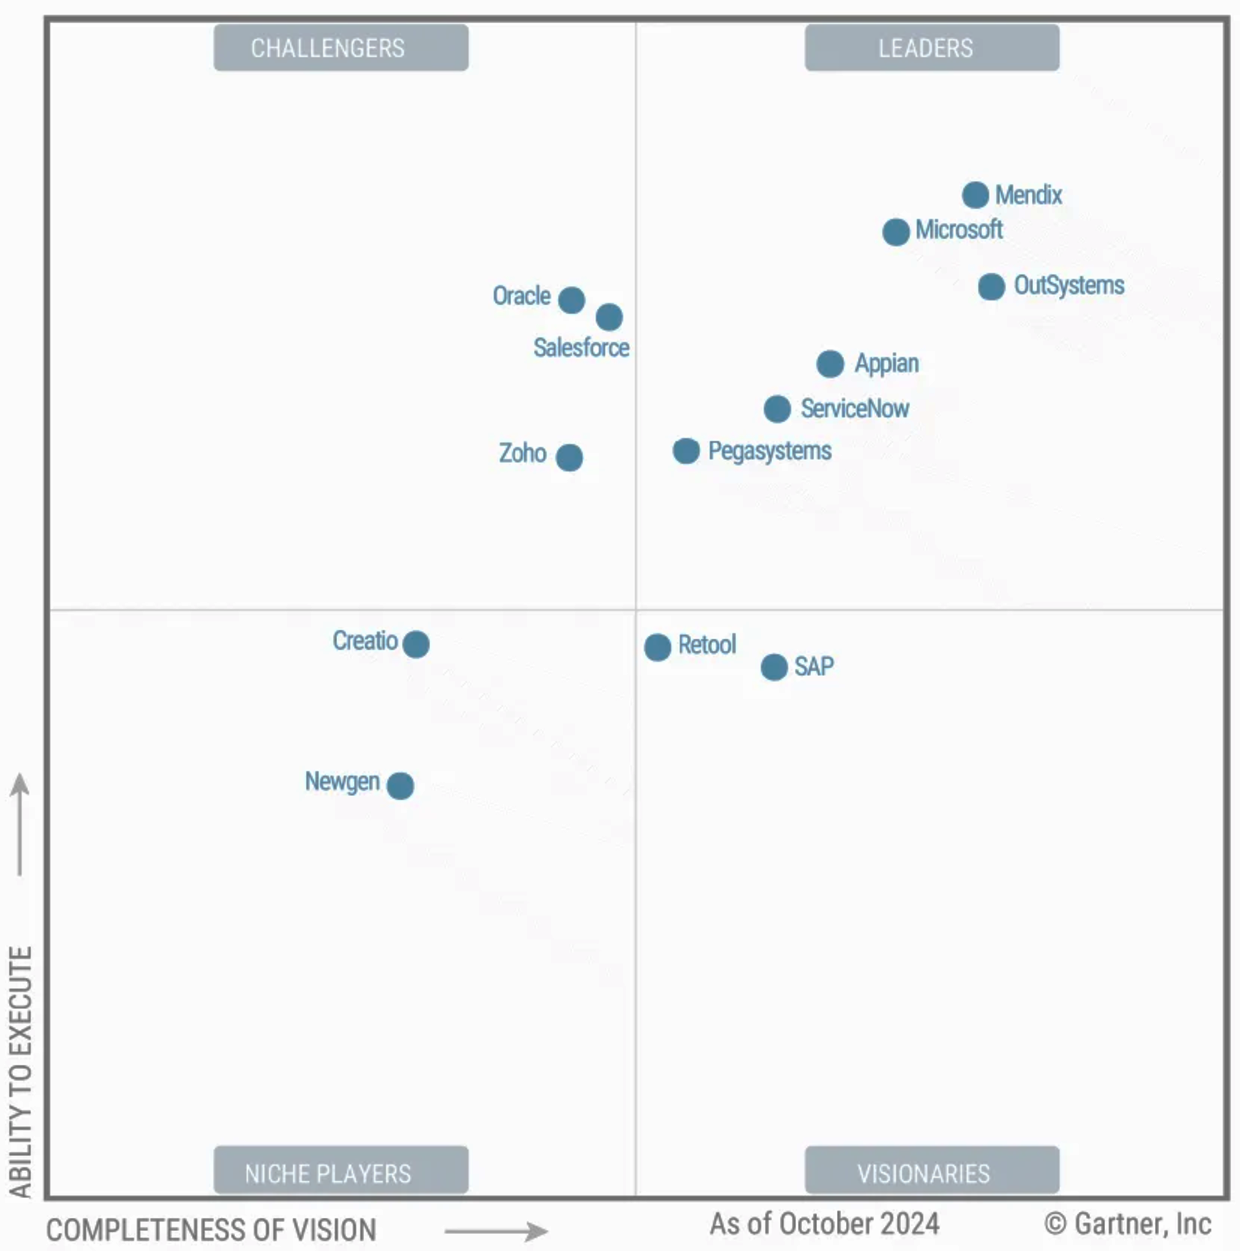
\includegraphics[width=0.5\textwidth]{GartnerQuadrant}
                    \caption{\centering Τεταρτημόριο της Gartner με πλατφόρμες ανάπτυξης λογισμικού \cite{mendixGartnerQuadrant}}
            \end{figure}

